% Options for packages loaded elsewhere
\PassOptionsToPackage{unicode}{hyperref}
\PassOptionsToPackage{hyphens}{url}
\PassOptionsToPackage{dvipsnames,svgnames,x11names}{xcolor}
%
\documentclass[
  11,
  a4paperpaper,
]{article}

\usepackage{amsmath,amssymb}
\usepackage{setspace}
\usepackage{iftex}
\ifPDFTeX
  \usepackage[T1]{fontenc}
  \usepackage[utf8]{inputenc}
  \usepackage{textcomp} % provide euro and other symbols
\else % if luatex or xetex
  \usepackage{unicode-math}
  \defaultfontfeatures{Scale=MatchLowercase}
  \defaultfontfeatures[\rmfamily]{Ligatures=TeX,Scale=1}
\fi
\usepackage{lmodern}
\ifPDFTeX\else  
    % xetex/luatex font selection
  \setmainfont[]{Arial}
\fi
% Use upquote if available, for straight quotes in verbatim environments
\IfFileExists{upquote.sty}{\usepackage{upquote}}{}
\IfFileExists{microtype.sty}{% use microtype if available
  \usepackage[]{microtype}
  \UseMicrotypeSet[protrusion]{basicmath} % disable protrusion for tt fonts
}{}
\makeatletter
\@ifundefined{KOMAClassName}{% if non-KOMA class
  \IfFileExists{parskip.sty}{%
    \usepackage{parskip}
  }{% else
    \setlength{\parindent}{0pt}
    \setlength{\parskip}{6pt plus 2pt minus 1pt}}
}{% if KOMA class
  \KOMAoptions{parskip=half}}
\makeatother
\usepackage{xcolor}
\usepackage[top=25mm,left=25mm,right=25mm,bottom=20mm,heightrounded]{geometry}
\setlength{\emergencystretch}{3em} % prevent overfull lines
\setcounter{secnumdepth}{5}
% Make \paragraph and \subparagraph free-standing
\ifx\paragraph\undefined\else
  \let\oldparagraph\paragraph
  \renewcommand{\paragraph}[1]{\oldparagraph{#1}\mbox{}}
\fi
\ifx\subparagraph\undefined\else
  \let\oldsubparagraph\subparagraph
  \renewcommand{\subparagraph}[1]{\oldsubparagraph{#1}\mbox{}}
\fi


\providecommand{\tightlist}{%
  \setlength{\itemsep}{0pt}\setlength{\parskip}{0pt}}\usepackage{longtable,booktabs,array}
\usepackage{calc} % for calculating minipage widths
% Correct order of tables after \paragraph or \subparagraph
\usepackage{etoolbox}
\makeatletter
\patchcmd\longtable{\par}{\if@noskipsec\mbox{}\fi\par}{}{}
\makeatother
% Allow footnotes in longtable head/foot
\IfFileExists{footnotehyper.sty}{\usepackage{footnotehyper}}{\usepackage{footnote}}
\makesavenoteenv{longtable}
\usepackage{graphicx}
\makeatletter
\def\maxwidth{\ifdim\Gin@nat@width>\linewidth\linewidth\else\Gin@nat@width\fi}
\def\maxheight{\ifdim\Gin@nat@height>\textheight\textheight\else\Gin@nat@height\fi}
\makeatother
% Scale images if necessary, so that they will not overflow the page
% margins by default, and it is still possible to overwrite the defaults
% using explicit options in \includegraphics[width, height, ...]{}
\setkeys{Gin}{width=\maxwidth,height=\maxheight,keepaspectratio}
% Set default figure placement to htbp
\makeatletter
\def\fps@figure{htbp}
\makeatother
% definitions for citeproc citations
\NewDocumentCommand\citeproctext{}{}
\NewDocumentCommand\citeproc{mm}{%
  \begingroup\def\citeproctext{#2}\cite{#1}\endgroup}
\makeatletter
 % allow citations to break across lines
 \let\@cite@ofmt\@firstofone
 % avoid brackets around text for \cite:
 \def\@biblabel#1{}
 \def\@cite#1#2{{#1\if@tempswa , #2\fi}}
\makeatother
\newlength{\cslhangindent}
\setlength{\cslhangindent}{1.5em}
\newlength{\csllabelwidth}
\setlength{\csllabelwidth}{3em}
\newenvironment{CSLReferences}[2] % #1 hanging-indent, #2 entry-spacing
 {\begin{list}{}{%
  \setlength{\itemindent}{0pt}
  \setlength{\leftmargin}{0pt}
  \setlength{\parsep}{0pt}
  % turn on hanging indent if param 1 is 1
  \ifodd #1
   \setlength{\leftmargin}{\cslhangindent}
   \setlength{\itemindent}{-1\cslhangindent}
  \fi
  % set entry spacing
  \setlength{\itemsep}{#2\baselineskip}}}
 {\end{list}}
\usepackage{calc}
\newcommand{\CSLBlock}[1]{\hfill\break#1\hfill\break}
\newcommand{\CSLLeftMargin}[1]{\parbox[t]{\csllabelwidth}{\strut#1\strut}}
\newcommand{\CSLRightInline}[1]{\parbox[t]{\linewidth - \csllabelwidth}{\strut#1\strut}}
\newcommand{\CSLIndent}[1]{\hspace{\cslhangindent}#1}

\let\oldsection\section
\renewcommand\section{\clearpage\oldsection}
\usepackage[font=it,labelfont=bf]{caption}
\makeatletter
\makeatother
\makeatletter
\makeatother
\makeatletter
\@ifpackageloaded{caption}{}{\usepackage{caption}}
\AtBeginDocument{%
\ifdefined\contentsname
  \renewcommand*\contentsname{Table of contents}
\else
  \newcommand\contentsname{Table of contents}
\fi
\ifdefined\listfigurename
  \renewcommand*\listfigurename{List of Figures}
\else
  \newcommand\listfigurename{List of Figures}
\fi
\ifdefined\listtablename
  \renewcommand*\listtablename{List of Tables}
\else
  \newcommand\listtablename{List of Tables}
\fi
\ifdefined\figurename
  \renewcommand*\figurename{Figure}
\else
  \newcommand\figurename{Figure}
\fi
\ifdefined\tablename
  \renewcommand*\tablename{Table}
\else
  \newcommand\tablename{Table}
\fi
}
\@ifpackageloaded{float}{}{\usepackage{float}}
\floatstyle{ruled}
\@ifundefined{c@chapter}{\newfloat{codelisting}{h}{lop}}{\newfloat{codelisting}{h}{lop}[chapter]}
\floatname{codelisting}{Listing}
\newcommand*\listoflistings{\listof{codelisting}{List of Listings}}
\makeatother
\makeatletter
\@ifpackageloaded{caption}{}{\usepackage{caption}}
\@ifpackageloaded{subcaption}{}{\usepackage{subcaption}}
\makeatother
\makeatletter
\makeatother
\ifLuaTeX
\usepackage[bidi=basic]{babel}
\else
\usepackage[bidi=default]{babel}
\fi
\babelprovide[main,import]{english}
\ifPDFTeX
\else
\babelfont{rm}[]{Arial}
\fi
% get rid of language-specific shorthands (see #6817):
\let\LanguageShortHands\languageshorthands
\def\languageshorthands#1{}
\ifLuaTeX
  \usepackage{selnolig}  % disable illegal ligatures
\fi
\IfFileExists{bookmark.sty}{\usepackage{bookmark}}{\usepackage{hyperref}}
\IfFileExists{xurl.sty}{\usepackage{xurl}}{} % add URL line breaks if available
\urlstyle{same} % disable monospaced font for URLs
\hypersetup{
  pdftitle={socioeconomic disruption by artificial intelligence},
  pdflang={en},
  colorlinks=true,
  linkcolor={blue},
  filecolor={Maroon},
  citecolor={Blue},
  urlcolor={Blue},
  pdfcreator={LaTeX via pandoc}}

\title{socioeconomic disruption by artificial intelligence}
\usepackage{etoolbox}
\makeatletter
\providecommand{\subtitle}[1]{% add subtitle to \maketitle
  \apptocmd{\@title}{\par {\large #1 \par}}{}{}
}
\makeatother
\subtitle{A comparative analysis between industries in the European
Union}
\author{}
\date{}

\begin{document}
\maketitle
\setstretch{1.5}
\pagenumbering{Roman}

\newpage{}

\tableofcontents

\newpage{}

\listoffigures

\newpage{}

\listoftables

\newpage{}

\pagenumbering{arabic}

\section{Abstract}\label{abstract}

\section{Introduction}\label{introduction}

Mokyr et al. (\citeproc{ref-mokyr_history_2015}{2015, p. 32}) identifies
two forms of technological anxiety, the fear of labor displacement
through technology and and the fear of morally negative applications
resulting in declining welfare. The majority of the US population has
been found to assess the potential impact of automation as unfavorable
rather than beneficial
(\citeproc{ref-anderson_automation_2017}{Anderson, 2017}).

Since AI is a still fairly new topic in the literature and has only seen
real increase in dominance and interest in recent years
(\citeproc{ref-acemoglu_ai_2020}{Acemoglu et al., 2020a, p. 23f}.), is
is worth noting the effects of previous technologies as the adoption of
machines (specifically often industrial robots
(\citeproc{ref-acemoglu_robots_2020}{Acemoglu and Restrepo, 2020a}; see
for example
\citeproc{ref-graetz_robots_2015}{\textbf{graetz\_robots\_2015?}})) and
software (also referred to as
computerization(\citeproc{ref-autor_growth_2013}{Autor and Dorn, 2013};
\citeproc{ref-frey_future_2017}{Frey and Osborne, 2017}; see for example
\citeproc{ref-pajarinen_computerization_2015}{Pajarinen et al., 2015}))
have been seen as previous stages in the evolution of automation with AI
composing the next stage (\citeproc{ref-acemoglu_harms_2021}{Acemoglu,
2021, p. 19}). Furthermore, these technologies have been summarized
under the umbrella term ``automation''
(\citeproc{ref-mann_benign_2018}{Mann and Püttmann, 2018, p. 40})
indicating common characteristics and thereby - possibly - common
effects.

\subsection{Effects of Automation on
labor}\label{effects-of-automation-on-labor}

In a 2018 study, the introduction of automation technology was found to
have positive effects on employment gains, but only within the same
commuting zone (\citeproc{ref-mann_benign_2018}{Mann and Püttmann, 2018,
p. 26}). These findings contradict the results from Autor et al.
(\citeproc{ref-autor_untangling_2015}{2015}) {[}p.~632{]}, that found no
relation between exposure to automation and employment as a whole but
found a significant decline in employment related to routine tasks in
the non-manufacturing sector (p.~641).
(\citeproc{ref-graetz_robots_2015}{\textbf{graetz\_robots\_2015?}})
found no relationship between the usage of industrial robots and net
employment. However, usage of industrial robots was found to lower
employment of low-skilled workers. However, a later study also looking
at employment effects induced by usage of industrial robots found a
significant decline of employment as well as a reduction in wages
related to robot exposure within a commuting zone
(\citeproc{ref-acemoglu_robots_2020}{Acemoglu and Restrepo, 2020a, pp.
2215f, 2218}). Dauth et al. (\citeproc{ref-dauth_german_2017}{2017})
{[}p.~25{]} found no relation between robot exposure and employment in
the German market. A few years later, Dauth et al.
(\citeproc{ref-dauth_adjustment_2021}{2021, p. 3126ff}) found robot
exposure to lead to within-firm and between-firm job displacement, with
displaced workers having difficulties reallocating their jobs within the
same industry, leading to a migration of workers from manufacturing
(where robot exposure is most present) to the service sector. They also
exhibited that a lack of worker protections (for example unionization or
tenure) is related to greater displacement. These results were also
confirmed by Boustan et al.
(\citeproc{ref-boustan_automation_2022}{2022}) {[}p.~21, 23{]} who
observed that displaced workers acquire new skills and concluded job
displacement by automation to be less discernible amongst unionized and
high-skilled workers. Similarily, Acemoglu and Restrepo
(\citeproc{ref-acemoglu_robots_2020}{2020a, p. 2215f}., 2218) provided
evidence showing automation (adoption of industrial robots) within a
commuting zone (local labor market) relating to significant declines in
employment as well as wages. By studying 53 developing countries, Cirera
and Sabetti (\citeproc{ref-cirera_effects_2019}{2019, p. 172}) did not
find a relationship between exposure to automation and firm level
employment. Hoewever, while a net effect on employment was absent, in
line with the aforementioned literature, they did find automation to
alter the composition of tasks and skills within firms (p.~172).

In a purely theoretical approach to the effects of automation on labor,
Acemoglu and Restrepo (\citeproc{ref-acemoglu_low-skill_2017}{2017})
{[}p.~12, 15{]} concluded that automation leads to labor displacement
and the displacement of low skilled-labor leading to an increase in the
wage gap (pay gap between low-skilled and high-skilled workers) while
the displacement of high-skilled labor is followed by a reduction in the
wage gap as high-skill labor reallocates into medium- and low-skilled
occupations. This reallocation from displaced high-skill labor into
lower skilled occupations has also been shown by Beaudry et al.
(\citeproc{ref-beaudry_great_2016}{2016, p. 21}) who studied the effects
on labor when prices for specific types of labor fall - as is induced
when substitution (through technology) becomes economically viable.
While labor displacement induced by the introduction of automation is
followed by increased inequality between low-skill and high-skilled
labor in the short run (\citeproc{ref-acemoglu_race_2018}{Acemoglu and
Restrepo, 2018a, p. 1519}), the creation of new tasks - that is followed
by increased productivity gains from automation - is seen to reduce this
gap in the long run (p.~1521). However, this positive outlook of a net
positive on employment only holds true as long as the productivity
effects which accompany the adoption of automation technologies offset
the displacement effects incurred in the first place - and should the
offset be insufficient, automation is found to negatively impact the
demand for labor and its wages
(\citeproc{ref-acemoglu_artificial_2018}{Acemoglu and Restrepo, 2018b,
p. 227}). There is also growing evidence suggesting automation to cause
a decline in real wages of low-skilled workers, for example Acemoglu and
Restrepo (\citeproc{ref-acemoglu_unpacking_2020}{2020b}) {[}p.~360f.{]}
found strong relationships between the adoption of automation technology
and wages. Acemoglu and Restrepo
(\citeproc{ref-acemoglu_tasks_2022}{2022, p. 1993}) found a relationship
between labor displacement and a decrease in relative wages, concluding
automation to cause an increase in wage inequality (p.~1998). Automation
is also attributed to the decline in the demand for labor in the US over
recent decades (\citeproc{ref-acemoglu_automation_2019}{Acemoglu and
Restrepo, 2019, p. 21}).

Furthermore, Arntz et al. (\citeproc{ref-arntz_risk_2016}{2016})
{[}p.~14f.{]} studying 21 OECD countries found 9\% in the US, and over
all countries studies a 6-12\% high risk of employment to be
substitutable for automation, while
(\citeproc{ref-acemoglu_chapter_2011}{\textbf{acemoglu\_chapter\_2011?}})
came to the conclusion that labor displacement by machines mostly
affects routine tasks.

\subsection{Effects of
computerization}\label{effects-of-computerization}

In a study from Finland, Pajarinen et al.
(\citeproc{ref-pajarinen_computerization_2015}{2015}) found that
computerization is likely to place high risk of displacement on 35\% of
the Finish labor market {[}p.~5{]}, 33\% of Norwegian labor (p.~5) as
well as 49\% in the US {[}p.~5{]}. Frey and Osborne
(\citeproc{ref-frey_future_2017}{2017, p. 41}) found 47\% of US
employment to have a a high risk suitability for substitution by
computerization. They further classify the process of automation into
two ``waves'' with the first wave affecting routine tasks
(transportation, logistics, office, and administration) {[}p.~41{]}
followed by a second wave that, once technological obstacles are
overcome, will effect the jobs involving creative or abstract tasks
{[}p.~43{]}. Evidence also suggests computerization to significantly
induce labor displacement from occupations relying on routine tasks into
higher-skilled occupations as well as low-skilled service occupations
(\citeproc{ref-autor_growth_2013}{Autor and Dorn, 2013, p. 1573})

\subsection{Effects of AI}\label{effects-of-ai}

Brynjolfsson et al. (\citeproc{ref-brynjolfsson_what_2018}{2018})
{[}p.~46{]} found that machine learning affects different types of tasks
than earlier forms of automation. A year later, in a study comparing the
impact of AI on the job market between industries, Webb
(\citeproc{ref-webb_impact_2019}{2019, p. 46}) shows that AI affects
mostly the highly educated workforce and that this group is affected
significantly more by AI than the presence of software or robots. Under
the assumption that the current trend in technological evolution is set
to continue, the speed of labor displacement through technological
innovation is found likely to outpace the speed at which labor can be
relocated (\citeproc{ref-mokyr_history_2015}{Mokyr et al., 2015, p.
43f}.). By constructing impact scores of Artificial Intelligence on
occupations, Felten et al. (\citeproc{ref-felten_effect_2019}{2019})
found low-income occupations to experience a decline in wage growth that
is attributed to the increased presence of AI and middle and high-income
occupations to experience an increase in wage growth {[}p.~6{]}.
Furthermore, the authors found found that occupations with a medium and
high degree of automation (degree of automation being the presence of
automation technologies - not just AI) positively correlate with
employment when exposed to Artificial Intelligence, while they did not
find any relationship for occupations already exhibiting a low degree of
automation {[}p.~5{]}.

It has also been noted that the presence of Artificial Intelligence does
not have a linear impact on labor but depends on influencing factors,
such as price elasticity, complementarities, or elasticity of labor that
govern the implementation of these technologies
(\citeproc{ref-brynjolfsson_what_2017}{Brynjolfsson and Mitchell, 2017,
p. 1533f}.). Additionally, the adoption of AI technology is found to
significantly alter the skill-demand distribution of firms, with the
number of previously highly demanded skills declining while
simultaneously creating demand for new skills
(\citeproc{ref-acemoglu_ai_2020}{Acemoglu et al., 2020a, p. 19}).

\subsection{Changes of Occupational composition (no net displacement but
need to
re-skill)}\label{changes-of-occupational-composition-no-net-displacement-but-need-to-re-skill}

Furthermore, it is important to note that previous research on the
effects of robots, software and AI - that have been summarized under the
umbrella term ``automation'' (\citeproc{ref-mann_benign_2018}{Mann and
Püttmann, 2018, p. 40}) - in general may not have found net negative
effects on employment but a restructuring of composition of occupations.
The aforementioned study from Autor et al.
(\citeproc{ref-autor_untangling_2015}{2015}) {[}p.~644{]} found
automation, while having no aggregate effects on employment, lead to a
decline in occupations involving routine tasks and and an increase in
non-routine (abstract) tasks. The same effect was found in
(\citeproc{ref-graetz_robots_2015}{\textbf{graetz\_robots\_2015?}})
studying the introduction of industrial robots.\\
These effects remain only harmless as long as the assumption holds true
that displaced labor can in fact always reallocate itself to new tasks.
Should this assumption be contradicted, and the the negative effects of
automation on employment are no longer offset by the positive effects of
reallocation, the phenomenon of occupational migration would turn into
an observation of job destruction.

\subsection{Changes in labor share}\label{changes-in-labor-share}

The introduction of capital, whether to complement or substitute labor,
intuitively leads to a decline of a firms profits paid to labor as the
share of labors input relative to the output value decreases. And in
fact Karabarbounis and Neiman
(\citeproc{ref-karabarbounis_global_2014}{2014}) {[}p.~99{]} show that
the observed decline in capital prices explains almost half the decline
in global labor share, that has been observed in recent decades. This
might seem problematic as an increasing portion of a firms revenue
remains as corporate profits and savings (given that the capital
invested leads to a decrease in marginal costs - through substitution of
labor and/ or increased production) rather than being redistributed to
labor. Karabarbounis and Neiman
(\citeproc{ref-karabarbounis_global_2014}{2014, p. 102}) further show
that the observed decline in labor share is accompanied by an increase
in corporate revenue and savings. This is also brought forward from
Acemoglu and Restrepo (\citeproc{ref-acemoglu_automation_2019}{2019})
{[}p.~27{]} who conclude that ``{[}\ldots{]} automation always reduces
the labor share and may reduce labor demand {[}\ldots{]}'' but also
mention that the creation of new tasks necessarily increases the labor
share. These results where further solidified by Acemoglu et al.
(\citeproc{ref-acemoglu_competing_2020}{2020b, p. 387}) who investigated
the French manufacturing market and found firms exposed to automation
(in this study measured by the introduction of robots) to experience
significant declines in their labor share.

\subsection{Summary of the different findings -\textgreater{} why
findings
differ}\label{summary-of-the-different-findings---why-findings-differ}

The net impact assessment of automation on socioeconomic factors widely
differs in the aforementioned literature (see also
\citeproc{ref-frank_toward_2019}{Frank et al., 2019, p. 6532}). Some
research has focused on local labor markets (commuting zones) (see
\citeproc{ref-acemoglu_robots_2020}{Acemoglu and Restrepo, 2020a};
\citeproc{ref-autor_untangling_2015}{Autor et al., 2015};
\citeproc{ref-autor_growth_2013}{Autor and Dorn, 2013}), while other
research has researched national effects {[}see xxx{]} and international
effects (see \citeproc{ref-graetz_robots_2018}{Graetz and Michaels,
2018}). While one would expect to see the same relationship between the
chosen variables on all levels and apart from differences in research
design, it may be difficult to assess effects on a greater aggregate
level as the number of variables that would need to be included to
account for differences between and within groups becomes unfeasible.

\subsection{Definitions of AI}\label{definitions-of-ai}

The classification if Artificial Intelligence remains also difficult due
to the fact that there is yet no widespread agreement on the definition
of intelligence itself (\citeproc{ref-legg_collection_2007}{Legg and
Hutter, 2007}).

\section{Methodology}\label{methodology}

The methodological approach has similarities to Mann and Püttmann
(\citeproc{ref-mann_benign_2018}{2018, p. 13}) who used patent counts as
a proxy for estimating the level of automation present within a US
commuting zone. However, the method of selecting patents differs. While
Mann and Püttmann (\citeproc{ref-mann_benign_2018}{2018}) classified
texts based on the tasks they may effect within occupations, the
presented approach here uses API query composition to preselect patents
whose title or abstract match keywords reserved to an industry.

\subsection{Data Sources}\label{data-sources}

Data about patent publications is obtained from the European Patent
Office's Open Patent Services (OPS) API
(\citeproc{ref-european_patent_office_open_2023}{European Patent Office,
2023}) as well as the Annual Structural Business Statistics (SBS) by
Eurostat (\citeproc{ref-eurostat_annual_2023}{Eurostat, 2023a}).
Furthermore, Eurostats code lists of Statistical classification of
economic activities in the European Community (NACE Revision 2)
(\citeproc{ref-eurostat_statistical_2023}{Eurostat, 2023b}) (henceforth
``NACE'') and Economic Indicators for Eurostat's SBS
(\citeproc{ref-eurostat_economical_2023}{Eurostat, 2023c}). While there
are a variety of possible technologies that may fall under the umbrella
term ``Artificial Intelligence'', as this research aims to assess AI's
socioeconomic impact - which, if negative, falls into the governmental
realm - a legal definition of AI is preferable as a classifier.
Furthermore, it is arguable that the political definition is likely to
have the greatest (socio)economic impact in the near future due to
possible (and probable) regulation. As there is no legal definition yet
- at least in the EU - technologies listed in the European Commisions
latest proposal for the ``Artificial Intelligence Act{[}'s{]}''
(\citeproc{ref-european_commission_proposal_2021}{European Commission,
2021}) annex (\citeproc{ref-european_commission_annexes_202}{European
Commission, 202AD}) will be used.\footnote{While this proposal is not
  yet in effect, it is likely to be adopted in the near future and is
  therefore used as a proxy for a legal definition of AI.}

Additionally Cooperative Patent Classification (CPC) codes are used to
retrieve patents that utilize artificial intelligence technology. As
there is no clear mapping between the European Commission's definition
and CPC codes, classifications are chosen to the author's best
knowledge.

\setstretch{1}

\phantomsection\label{tbl-cpc-codes}
\begin{longtable}[]{@{}ll@{}}
\caption{\label{tbl-cpc-codes}Selected CPC Codes}\tabularnewline
\toprule\noalign{}
Class & CPC \\
\midrule\noalign{}
\endfirsthead
\toprule\noalign{}
Class & CPC \\
\midrule\noalign{}
\endhead
\bottomrule\noalign{}
\endlastfoot
Machine Learning & G06N20/00, G06N20/10, G06N20/20 \\
Supervised Learning & G06N3/09 \\
Unsupervised Learning & G06N3/088 \\
Reinforcement Learning & G06N3/092 \\
Deep Learning & G06N3/08 \\
\end{longtable}

\setstretch{1.5}

\subsection{Data Acquisition}\label{sec-data-acquisition}

In order to retrieve data from the European Patent Office's Open Patent
Services (OPS) API, queries were composed to link retrieved patents to
their respective industry. The query composition is based on the
selected CPC codes displayed in Table~\ref{tbl-cpc-codes} as well as
keywords from the list of NACE codes that have been retrieved from
Eurostat. Each NACE code is composed of section (alphabetical), division
(numerical), group (numerical) and class (numerical) of a particular
economic activity. Sections relate to the overall industry, while
divisions, groups and classes relate to more specific activities within
the industry (\citeproc{ref-nacebac}{\textbf{nacebac?}}). For each
industry, keywords are extracted from the NACE code's description. To
ensure only relevant keywords are used, each description is cleaned of
common characters and unrelated words (e.g., ``,'', ``and'', ``or'',
``to''). Descriptions for each industry are then split into lists of
single keywords that will be used in the API query.

Because some industries contain a variety of different activities (e.g.,
NACE industry (section) ``A'' relates to ``Agriculture, forestry and
fishing'' (\citeproc{ref-eurostat_economical_2023}{Eurostat, 2023c})),
main keywords that relate to the section as a whole are manually
selected (see Table~\ref{tbl-nacemainkeywords} in the
\nameref{sec-appendix}). For each industry and main keyword, queries are
then build using the (manuallly selected) main keyword, the description
keywords, as well as the chosen CPC codes. The resulting query is then
used to retrieve patents from the OPS API. To limit query results to the
relevant market, only patents filed with the European Patent Office (EP)
will be retrieved. This approach disregards patents filed with national
patent offices. However, since the query language is english, and many
national patents are only filed in their native language, retrieving
patents for all EU markets was unfeasible. The query is composed of the
following elements:

\begin{quote}
\textbf{(ta = Main Keyword) AND (ta = ANY Description Keywords) AND (cpc
ANY CPC Codes) AND (ap = ``EP'')}\\
\emph{Note: ta = title or abstract; ap = Application Number, referring
to the Patent Office the patent was filed at. In this case, ``EP''
refers to the European Patent Office. See Table~\ref{tbl-queryexample}
for example queries}
\end{quote}

The queries are then posted to the OPS API's Published Data Keywords
Search with Variable Constituents endpoint
(\citeproc{ref-european_patent_office_published_nodate}{European Patent
Office, n.d.}) and data from the responses - which are provided in JSON
format - extracted.

\subsection{Preprocessing}\label{sec-preprocessing}

Since Eurostat's SBS data only includes codes to refer to given
indicators as well as industries, data retrieved from Eurostat (SBS, and
Code Lists about NACE and SBS codes) is merged. This is done by matching
the NACE codes and SBS indicator codes to the respective NACE code and
indicator in the SBS data. The economic indicators ``Enterprises'' and
``Persons employed'' are reported as totals. ``Wage adjusted labour
productivity (Apparent labour productivity by average personnel costs)''
and ``Share of personnel costs in production'' are reported as
percentages, and ``Gross value added per employee'' is reported in
Euros. Because the number of employees is rather large for each
industry, the number of employees is divided by 1000 to reduce the scale
of the data. This increases readability of tables in the following
regression results while also still large enough that it is unlikely for
coefficients (coeff.) and standard errors (SE) to fall too far into the
decimals.\footnote{Note that this is done to ensure readability and does
  not affect the regression results. Defactoring data by more than a
  thousand might lead to coefficients and standard errors falling into
  the decimals, which in turn may show up - due to rounding - as zeros
  despite having large scale effects (when rescaled with the original
  factor).\label{note3}}

Next, patent data retrieved from the OPS API, which returns data in JSON
format, is converted into a pandas DataFrame
(\citeproc{ref-the_pandas_development_team_pandas-devpandas_2023}{The
pandas development team, 2023}) (i.e., a table). As multiple queries for
the same industry - but with different keywords - have been posted to
the API, duplicates in the patent data are removed. Specifically,
duplicate patent data (indicated by the patent application number) are
removed in each industry subset of the data. This ensures that each
industry only contains unique patents while patents can still appear in
more than one industry (as their applicable usage may not be restricted
to only one industry). Furthermore, as the SBS data only spans from 2011
to 2020, patents that have been filed before or after this period are
removed from the data. As a next step, patents are grouped by their
respective industry and year of application and the patent count for
each subgroup is recorded. Furthermore, industries for which patents
have been retrieved in less than four years within 2011-2020 are removed
from the data to ensure a minimum sample size for the following
statistics. The sum of patents for each industry and year composes the
exogenous variable ``Sum patents'' that will be used in the regression
analyses.

Furthermore, the SBS data is merged with the patent data by matching the
industry and year of application with the industry and year of the SBS
data. This ensures that each industry and year combination in the SBS
data has a corresponding patent count. Furthermore, the data is once
more grouped for each industry to retrieve the earliest and latest year
for which patent counts are available. For each industry, SBS data is
removed for the years before and after the first and last patent
retrieval for the respective industry. This is done to ensure that the
regression analyses are only conducted for years in which patent counts
are available.\footnote{There are valid arguments to be made for and
  against excluding these data. For once, the lack of patent retrieval
  for any given year implies no patent filing within that year, making
  null values a good control instance to check for variation in SBS data
  that is definitely not affected by patent filings. On the other hand,
  for a few industries, this would result in many null values, giving
  the data series of patent counts a definite trend. Furthermore, patent
  counts have also been removed for years in which SBS data is
  unavailable. To reduce potential bias produced by imputing and keeping
  the data's integrity, removing the missing values has been chosen over
  the data's accuracy.} However, in some cases, patents were
discontinuously retrieved for industries. In other words, if patents are
retrieved for an industry in 2016, 2018, 2019, and 2020, but not in
2017, the SBS data for 2017 and the respective do not have a
corresponding patent count. In order to account for missing values
within a series of definite patent retrieval, the patent count for the
missing year is set to zero. This is done for each industry and year
combination in which patent counts are missing.

Lastly, in some rare cases, SBS data is missing for a given year and
industry. In these cases, rows of the respective year and industry are
removed from the data. This is done to ensure that the regression
analyses are only conducted for years in which SBS data is available.
The resulting data is then used for the regression analyses. In summary,
data for each year and industry will be used further if the following
conditions are met.

\begin{enumerate}
\def\labelenumi{\arabic{enumi}.}
\tightlist
\item
  Patents have been retrieved for the industry in at least four years
  within 2011-2020
\item
  Patents have been retrieved for this or an earlier year
\item
  Patents have been retrieved for this or a later year
\item
  SBS data is available for this year and industry
\end{enumerate}

The resulting data contains 211 data points across 6 Industries, each
with 5 economic indicators. However, given the relatively short time
period in which data could have been collected, paired with the fact
that the retrieved patents are aggregated for each year, the resulting
data size for each industry and economic indicator is relative small.
The average number of years in which patent counts have been recorded
-according to the methods above- is only 7 years, ranging from a minimum
of 4 years up to 10 years. Since each year per industry and indicator
will be used as a data point in the following regression analyses, it is
neccesary to note that results may be biased due to the small sample
size. Furthermore, given the small dataset -which makes diminishes the
accuracy with which a regression can be fitted (i.e., fewer ``anchor
points''), assumptions about the extend to which patent counts affect
the chosen economic indicators will not be made. Instead, the regression
analyses will be used to assess whether a relationship between the
number of patents and the chosen economic indicators exists at all. That
is, the interest lies whether AI patent counts yield any explanatory
power over the chosen economic indicators.

Because the collected data comrpises a time-series, as each industry's
patent application counts as well as the SBS data have been retrieved
for multiple years. As shown in
Figure~\ref{fig-untransformed-data-example}, the collected data on SBS
indicators (blue) as well as the number of patents retrieved each year
(red) clearly does not exhibit stationarity. In order to account for any
trends in the data, the collected data is transformed using linear
detrending method. This is done by utilicing scipy's detrending method
(\citeproc{ref-virtanen_scipy_2020}{Virtanen et al., 2020}), which fits
a linear least-squares regression to the data and subtracts the
resulting trend of the regression line from the data
(\citeproc{ref-the_scipy_community_scipysignaldetrend_2023}{The SciPy
community, 2023}). Note that other detrending options, such as
logarithmic transformation or differencing have been considered but
deemed insifficient. Logarithmic transformation is not applicable as the
data contains zero values. While there are methods to circumvent this,
for example taking the logarithm \(log(x+1)\), this would lead to
non-null values where null values are expected to control for variance
in the endogenous variable in the absence of patent counts. Furthermore,
as seen in Figure~\ref{fig-untransformed-data-example}, many data series
exhibit a continues positive or negative trend (a lack of fluctuation).
In this case, differencing would merely reverse the trend, and
logarithmic detrending would lead to a compression of the y-scale.
Resulting data transformed by either of these methods, however, would
still exhibit a definite trend. The resulting data, of which an example
is shown in Figure~\ref{fig-transformed-data-example}, is then used for
the regression analyses.

\begin{figure}[H]

{\centering 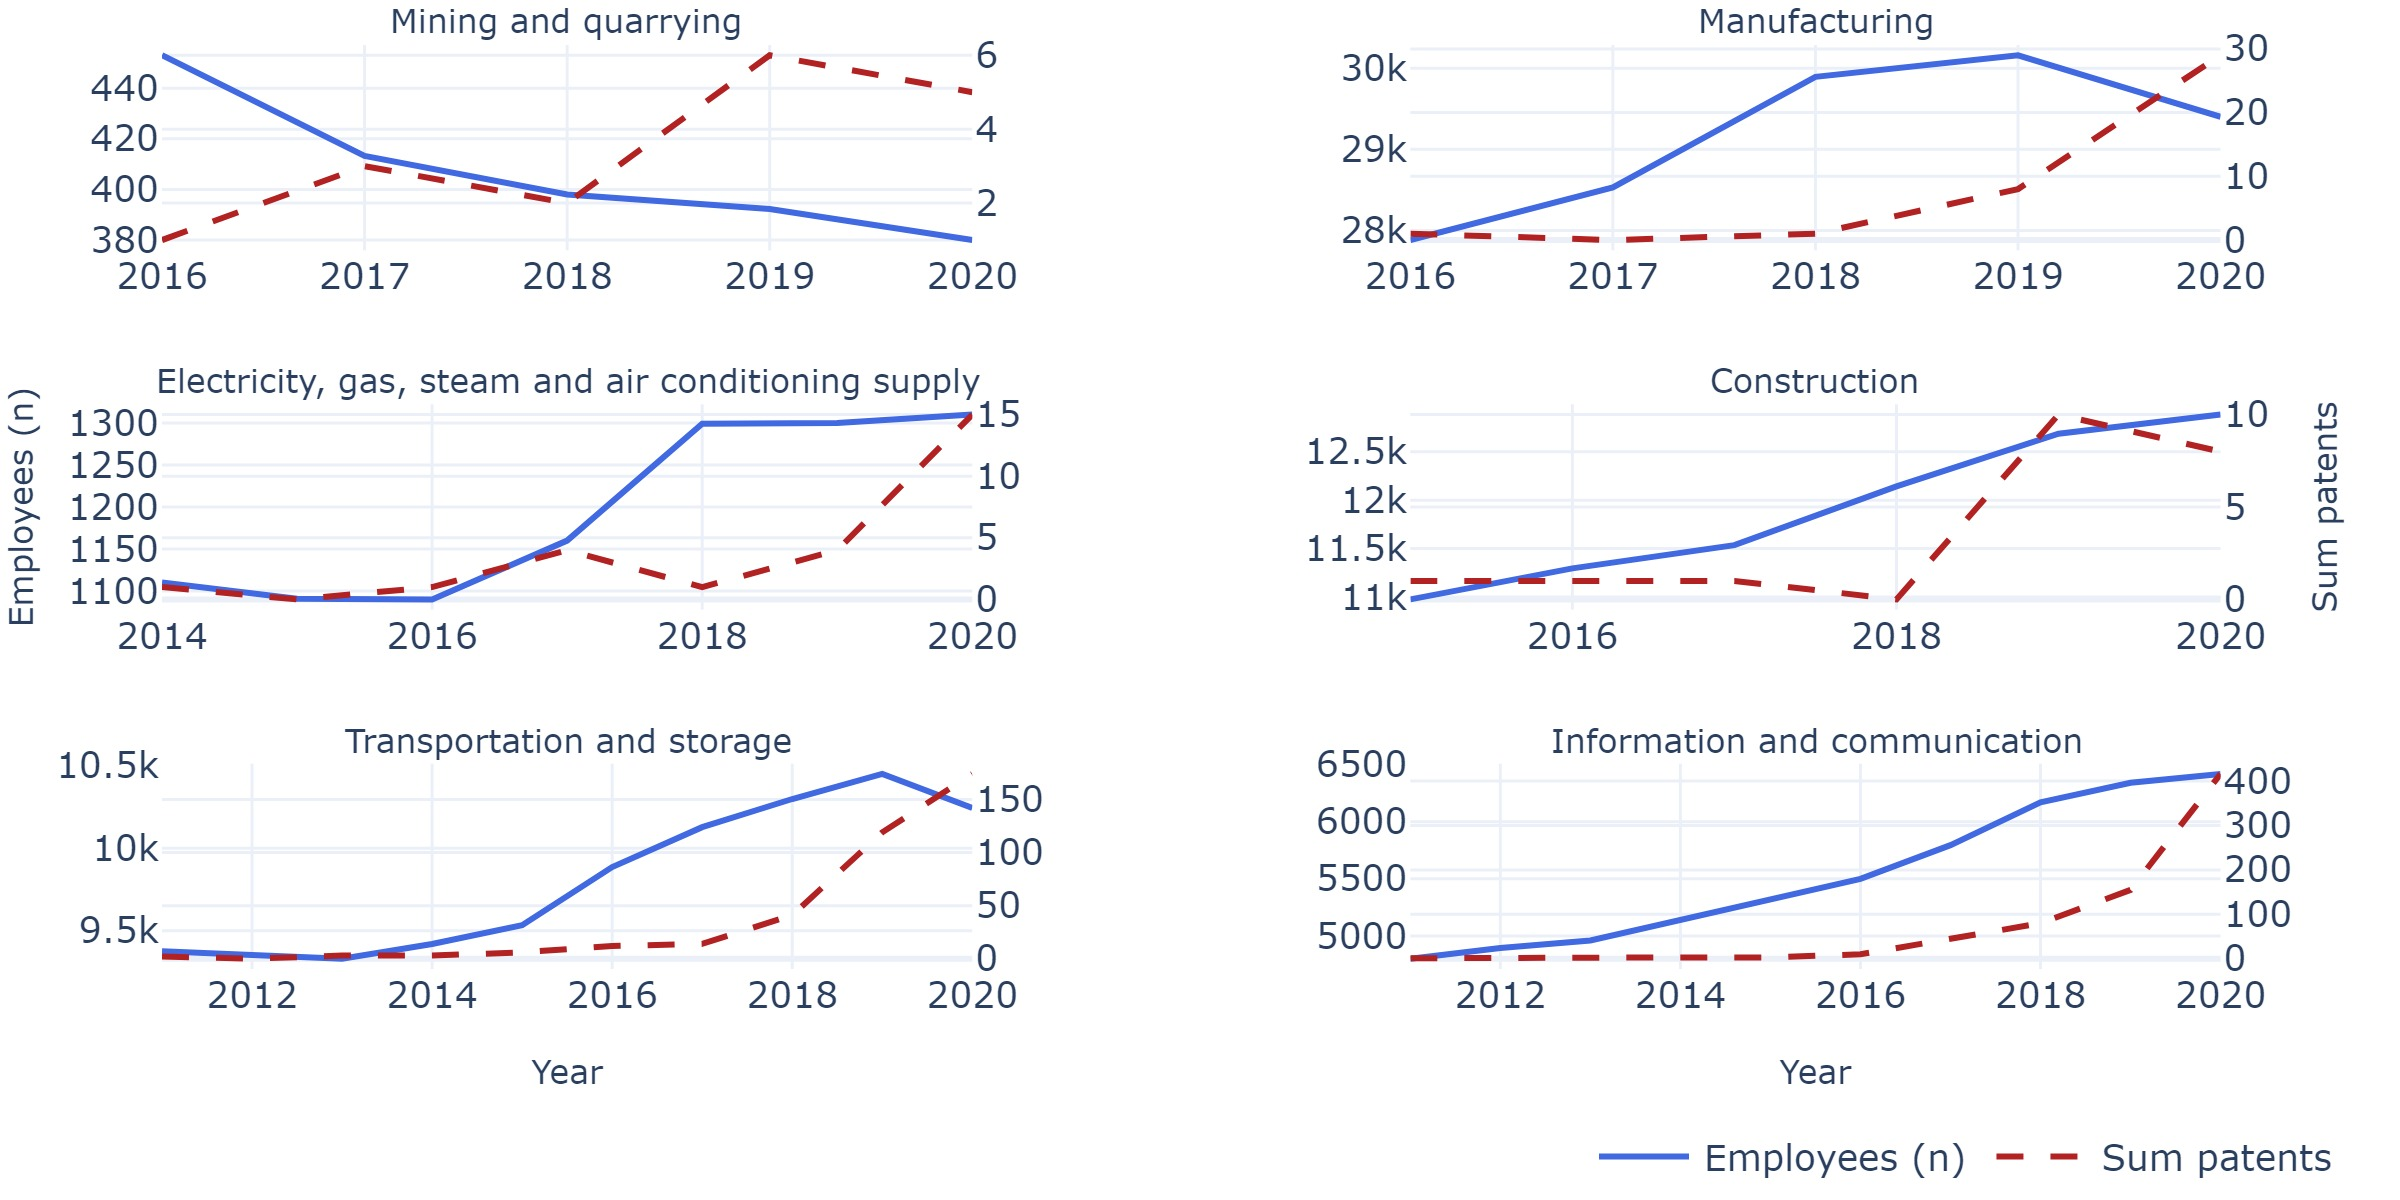
\includegraphics{rieg2023_files/figure-pdf/fig-untransformed-data-example-output-1.jpeg}

}

\caption{\label{fig-untransformed-data-example}Example of untransformed
data for all Industries and NACE Code `Number of Employees' plotted over
years}

\end{figure}

\begin{figure}[H]

{\centering 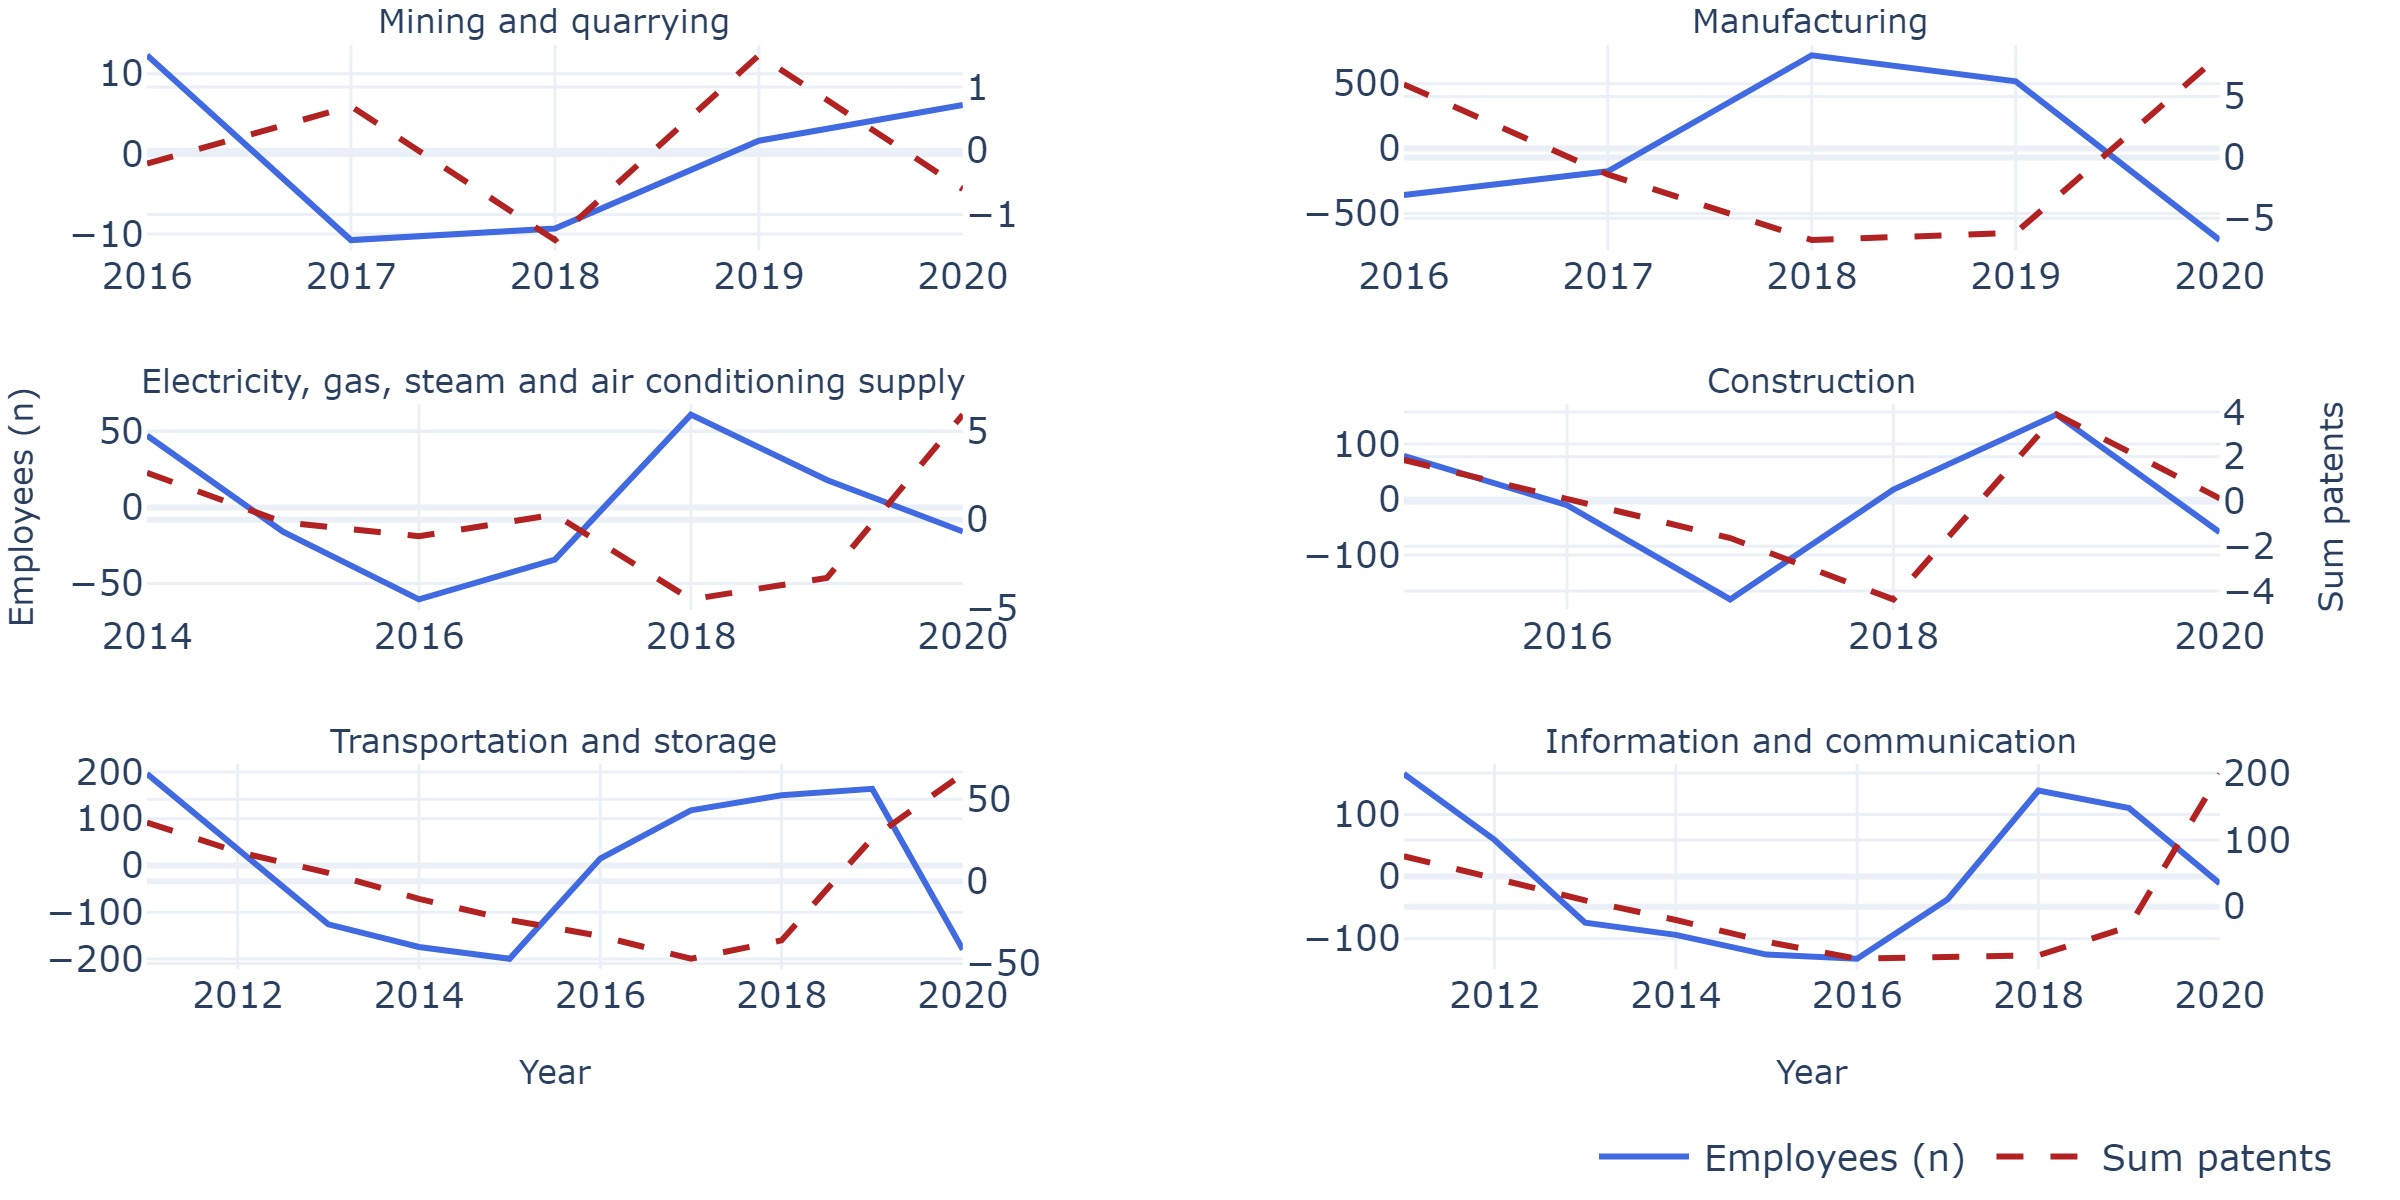
\includegraphics{rieg2023_files/figure-pdf/fig-transformed-data-example-output-1.jpeg}

}

\caption{\label{fig-transformed-data-example}Example of linear detrended
data for all Industries and NACE Code `Number of Employees' plotted over
years}

\end{figure}

Because data has been linearily detrended, to account for any remaining
trend left in the data, the control variable ``Year'' is added to the
regression analyses. This is done to ensure that any remaining trend in
the data is accounted for and does not bias the regression results.
Furthermore, the control variable ``Year'' is also added to the
regression analyses to account for any time dependent macroeconomic
effects that may have affected the chosen economic indicators but are
not considered in the model.

\subsection{Hypothesis}\label{hypothesis}

Do determine whether a relationship between the number of patents and
the chosen economic indicators exists, the following hypotheses are
tested. Given a standard multiple linear regression model of the form
\(ŷ_{ij} = \beta_0 + \beta_1x_i + + \beta_1x_t\), where
\(i=\text{industry, }j=\text{economic indicator }\text{and }t=\text{time}\),
the coefficient \(\beta_1\) is assumed to be \(0\). Specifically, the
following assumptions are tested. \begin{align}
H_0^{lb}: \beta_1 = 0\text{ for }y_{j=lb}=\text{wage adjusted labor productivity} \\
H_0^{pc}: \beta_1 = 0\text{ for }y_{j=pc}=\text{personnel costs in production} \\
H_0^{e}: \beta_1 = 0\text{ for }y_{j=e}=\text{number of employees} \\
H_0^{va}: \beta_1 = 0\text{ for }y_{j=va}=\text{gross value added per employee}
\end{align}

\section{Results}\label{results}

The following section presents the main findings from the regression
analyses. Results are summarized by industry, allowing a sectional
comparrison of patent counts' influence on economic indicators within an
industry.

\setstretch{1}

\phantomsection\label{tbl-regression-results-ind-b}
\begin{longtable}[]{@{}
  >{\raggedright\arraybackslash}p{(\columnwidth - 10\tabcolsep) * \real{0.1404}}
  >{\raggedright\arraybackslash}p{(\columnwidth - 10\tabcolsep) * \real{0.1667}}
  >{\raggedright\arraybackslash}p{(\columnwidth - 10\tabcolsep) * \real{0.1491}}
  >{\raggedright\arraybackslash}p{(\columnwidth - 10\tabcolsep) * \real{0.1667}}
  >{\raggedright\arraybackslash}p{(\columnwidth - 10\tabcolsep) * \real{0.1754}}
  >{\raggedright\arraybackslash}p{(\columnwidth - 10\tabcolsep) * \real{0.2018}}@{}}
\caption{\label{tbl-regression-results-ind-b}Regression results - Mining
and Quarrying (B)}\tabularnewline
\toprule\noalign{}
\begin{minipage}[b]{\linewidth}\raggedright
\end{minipage} & \begin{minipage}[b]{\linewidth}\raggedright
Enterprises (n)
\end{minipage} & \begin{minipage}[b]{\linewidth}\raggedright
Employees (n)
\end{minipage} & \begin{minipage}[b]{\linewidth}\raggedright
Labor prod. (\%)
\end{minipage} & \begin{minipage}[b]{\linewidth}\raggedright
GVA/employee (€)
\end{minipage} & \begin{minipage}[b]{\linewidth}\raggedright
Personnel costs (\%)
\end{minipage} \\
\midrule\noalign{}
\endfirsthead
\toprule\noalign{}
\begin{minipage}[b]{\linewidth}\raggedright
\end{minipage} & \begin{minipage}[b]{\linewidth}\raggedright
Enterprises (n)
\end{minipage} & \begin{minipage}[b]{\linewidth}\raggedright
Employees (n)
\end{minipage} & \begin{minipage}[b]{\linewidth}\raggedright
Labor prod. (\%)
\end{minipage} & \begin{minipage}[b]{\linewidth}\raggedright
GVA/employee (€)
\end{minipage} & \begin{minipage}[b]{\linewidth}\raggedright
Personnel costs (\%)
\end{minipage} \\
\midrule\noalign{}
\endhead
\bottomrule\noalign{}
\endlastfoot
const & 0.000 & 0.000 & -0.000 & -3878292.052 & 0.000 \\
& (119814.660) & (8940.246) & (32619.930) & (20665152.759) &
(998.515) \\
Sum patents & -88.647 & 0.363 & -8.145 & -1340.991 & 0.645 \\
& (83.139) & (6.204) & (22.635) & (14778.928) & (0.693) \\
Year & -0.000 & -0.000 & 0.000 & 1921.611 & -0.000 \\
& (59.373) & (4.430) & (16.164) & (10239.141) & (0.495) \\
R-squared & 0.362 & 0.002 & 0.061 & 0.041 & 0.302 \\
R-squared Adj. & -0.275 & -0.997 & -0.878 & -1.877 & -0.395 \\
\end{longtable}

\setstretch{1.5}

For patents classified as industry ``Mining and Quarrying'' (NACE code
``B''), depicted in Table~\ref{tbl-regression-results-ind-b}, the
regression results show no significant relation between the sum of
patents retrieved for each year and the chosen indicators. Furthermore,
the control variable ``Year'', too, does not exhibit any significant
relationships with the economic indicators. It should be noted, howver,
that the number of patents retrieved for this industry is very low.
While, as discussed in the \nameref{sec-data-acquisition}, industries
for which patents were retrieved in fewer than five years were
eliminated from the data, for Mining and Quarrying only 17.0 patents in
5 years were retrieved.

\setstretch{1}

\phantomsection\label{tbl-regression-results-ind-c}
\begin{longtable}[]{@{}
  >{\raggedright\arraybackslash}p{(\columnwidth - 10\tabcolsep) * \real{0.1404}}
  >{\raggedright\arraybackslash}p{(\columnwidth - 10\tabcolsep) * \real{0.1667}}
  >{\raggedright\arraybackslash}p{(\columnwidth - 10\tabcolsep) * \real{0.1491}}
  >{\raggedright\arraybackslash}p{(\columnwidth - 10\tabcolsep) * \real{0.1667}}
  >{\raggedright\arraybackslash}p{(\columnwidth - 10\tabcolsep) * \real{0.1754}}
  >{\raggedright\arraybackslash}p{(\columnwidth - 10\tabcolsep) * \real{0.2018}}@{}}
\caption{\label{tbl-regression-results-ind-c}Regression results -
Manufacturing (C)}\tabularnewline
\toprule\noalign{}
\begin{minipage}[b]{\linewidth}\raggedright
\end{minipage} & \begin{minipage}[b]{\linewidth}\raggedright
Enterprises (n)
\end{minipage} & \begin{minipage}[b]{\linewidth}\raggedright
Employees (n)
\end{minipage} & \begin{minipage}[b]{\linewidth}\raggedright
Labor prod. (\%)
\end{minipage} & \begin{minipage}[b]{\linewidth}\raggedright
GVA/employee (€)
\end{minipage} & \begin{minipage}[b]{\linewidth}\raggedright
Personnel costs (\%)
\end{minipage} \\
\midrule\noalign{}
\endfirsthead
\toprule\noalign{}
\begin{minipage}[b]{\linewidth}\raggedright
\end{minipage} & \begin{minipage}[b]{\linewidth}\raggedright
Enterprises (n)
\end{minipage} & \begin{minipage}[b]{\linewidth}\raggedright
Employees (n)
\end{minipage} & \begin{minipage}[b]{\linewidth}\raggedright
Labor prod. (\%)
\end{minipage} & \begin{minipage}[b]{\linewidth}\raggedright
GVA/employee (€)
\end{minipage} & \begin{minipage}[b]{\linewidth}\raggedright
Personnel costs (\%)
\end{minipage} \\
\midrule\noalign{}
\endhead
\bottomrule\noalign{}
\endlastfoot
const & 0.000 & 0.000 & -0.000 & -0.000 & 0.000 \\
& (15775939.211) & (161822.011) & (554.469) & (306669.659) &
(133.493) \\
Sum patents & -14.607 & -82.489** & -0.130 & -203.313** & 0.040 \\
& (1778.568) & (18.244) & (0.063) & (34.574) & (0.015) \\
Year & -0.000 & -0.000 & 0.000 & 0.000 & -0.000 \\
& (7817.609) & (80.189) & (0.275) & (151.967) & (0.066) \\
R-squared & 0.000 & 0.911 & 0.684 & 0.945 & 0.779 \\
R-squared Adj. & -1.000 & 0.822 & 0.368 & 0.891 & 0.558 \\
\end{longtable}

\setstretch{1.5}

For patents classified as industry ``Manufacturing'' (NACE code ``C''),
depicted in Table~\ref{tbl-regression-results-ind-c}, the regression
results show a statistically significant negative relationship between
the number of retrieved patents and the number of employees within the
Manufacturing sector (coeff. -82.488.8, SE 18.243`). In particular, the
regression result's coefficient estimates a decrease of 82489 employees
for each additional patent retrieved\footnote{Note that while the
  coefficient's implications are mentioned, this merely refers to the
  slope of the regression line and should not be interpreted as valid
  result with real-world implications. The regression model is not
  intended to be used for prediction.}. Furthermore, the control
variable ``Year'' does not exhibit a statistically significant
relationship with the number of employees (coeff. 0). The adjusted
\(R^2\) of 0.82 indicates a high ratio of explainability for the model.

While there are no statistically significant relations between the
number of patents retrieved and the number of enterprises, wage adjusted
labor productivity (labor prod.) and the percentage of personnel costs
in production, the relationship between the number of patents and the
gross value added per employee is statistically significant and negative
(coeff. -203.313, SE 34.574) with an adjustes \(R^2\) of 0.89. Lastly,
it should be noted that the control variable does not exhibit a
statistically significant relationship with any of the economic
indicators.

\setstretch{1}

\phantomsection\label{tbl-regression-results-ind-d}
\begin{longtable}[]{@{}
  >{\raggedright\arraybackslash}p{(\columnwidth - 10\tabcolsep) * \real{0.1404}}
  >{\raggedright\arraybackslash}p{(\columnwidth - 10\tabcolsep) * \real{0.1667}}
  >{\raggedright\arraybackslash}p{(\columnwidth - 10\tabcolsep) * \real{0.1491}}
  >{\raggedright\arraybackslash}p{(\columnwidth - 10\tabcolsep) * \real{0.1667}}
  >{\raggedright\arraybackslash}p{(\columnwidth - 10\tabcolsep) * \real{0.1754}}
  >{\raggedright\arraybackslash}p{(\columnwidth - 10\tabcolsep) * \real{0.2018}}@{}}
\caption{\label{tbl-regression-results-ind-d}Regression results -
Electricity, gas, steam and air conditioning supply (D)}\tabularnewline
\toprule\noalign{}
\begin{minipage}[b]{\linewidth}\raggedright
\end{minipage} & \begin{minipage}[b]{\linewidth}\raggedright
Enterprises (n)
\end{minipage} & \begin{minipage}[b]{\linewidth}\raggedright
Employees (n)
\end{minipage} & \begin{minipage}[b]{\linewidth}\raggedright
Labor prod. (\%)
\end{minipage} & \begin{minipage}[b]{\linewidth}\raggedright
GVA/employee (€)
\end{minipage} & \begin{minipage}[b]{\linewidth}\raggedright
Personnel costs (\%)
\end{minipage} \\
\midrule\noalign{}
\endfirsthead
\toprule\noalign{}
\begin{minipage}[b]{\linewidth}\raggedright
\end{minipage} & \begin{minipage}[b]{\linewidth}\raggedright
Enterprises (n)
\end{minipage} & \begin{minipage}[b]{\linewidth}\raggedright
Employees (n)
\end{minipage} & \begin{minipage}[b]{\linewidth}\raggedright
Labor prod. (\%)
\end{minipage} & \begin{minipage}[b]{\linewidth}\raggedright
GVA/employee (€)
\end{minipage} & \begin{minipage}[b]{\linewidth}\raggedright
Personnel costs (\%)
\end{minipage} \\
\midrule\noalign{}
\endhead
\bottomrule\noalign{}
\endlastfoot
const & 0.000 & 0.000 & -0.000 & 0.000 & 0.000 \\
& (7090398.833) & (19752.895) & (2819.369) & (1493538.845) &
(103.597) \\
Sum patents & -2148.926 & -3.428 & 1.436 & 581.888 & 0.044 \\
& (2160.274) & (6.018) & (0.859) & (455.045) & (0.016) \\
Year & -0.000 & -0.000 & 0.000 & -0.000 & -0.000 \\
& (3515.317) & (9.793) & (1.398) & (740.475) & (0.051) \\
R-squared & 0.198 & 0.075 & 0.411 & 0.290 & 0.878 \\
R-squared Adj. & -0.203 & -0.387 & 0.117 & -0.065 & 0.634 \\
\end{longtable}

\phantomsection\label{tbl-regression-results-ind-f}
\begin{longtable}[]{@{}
  >{\raggedright\arraybackslash}p{(\columnwidth - 10\tabcolsep) * \real{0.1404}}
  >{\raggedright\arraybackslash}p{(\columnwidth - 10\tabcolsep) * \real{0.1667}}
  >{\raggedright\arraybackslash}p{(\columnwidth - 10\tabcolsep) * \real{0.1491}}
  >{\raggedright\arraybackslash}p{(\columnwidth - 10\tabcolsep) * \real{0.1667}}
  >{\raggedright\arraybackslash}p{(\columnwidth - 10\tabcolsep) * \real{0.1754}}
  >{\raggedright\arraybackslash}p{(\columnwidth - 10\tabcolsep) * \real{0.2018}}@{}}
\caption{\label{tbl-regression-results-ind-f}Regression results -
Construction (F)}\tabularnewline
\toprule\noalign{}
\begin{minipage}[b]{\linewidth}\raggedright
\end{minipage} & \begin{minipage}[b]{\linewidth}\raggedright
Enterprises (n)
\end{minipage} & \begin{minipage}[b]{\linewidth}\raggedright
Employees (n)
\end{minipage} & \begin{minipage}[b]{\linewidth}\raggedright
Labor prod. (\%)
\end{minipage} & \begin{minipage}[b]{\linewidth}\raggedright
GVA/employee (€)
\end{minipage} & \begin{minipage}[b]{\linewidth}\raggedright
Personnel costs (\%)
\end{minipage} \\
\midrule\noalign{}
\endfirsthead
\toprule\noalign{}
\begin{minipage}[b]{\linewidth}\raggedright
\end{minipage} & \begin{minipage}[b]{\linewidth}\raggedright
Enterprises (n)
\end{minipage} & \begin{minipage}[b]{\linewidth}\raggedright
Employees (n)
\end{minipage} & \begin{minipage}[b]{\linewidth}\raggedright
Labor prod. (\%)
\end{minipage} & \begin{minipage}[b]{\linewidth}\raggedright
GVA/employee (€)
\end{minipage} & \begin{minipage}[b]{\linewidth}\raggedright
Personnel costs (\%)
\end{minipage} \\
\midrule\noalign{}
\endhead
\bottomrule\noalign{}
\endlastfoot
const & -0.000 & -0.000 & -0.000 & 0.000 & 0.000 \\
& (21172494.612) & (58291.431) & (659.644) & (476813.850) & (117.828) \\
Sum patents & 9252.711 & 23.444 & -0.236 & 16.501 & 0.019 \\
& (6911.846) & (19.029) & (0.215) & (155.658) & (0.038) \\
Year & 0.000 & 0.000 & 0.000 & -0.000 & -0.000 \\
& (10494.417) & (28.893) & (0.327) & (236.339) & (0.058) \\
R-squared & 0.374 & 0.336 & 0.285 & 0.004 & 0.076 \\
R-squared Adj. & -0.043 & -0.107 & -0.191 & -0.660 & -0.541 \\
\end{longtable}

\setstretch{1.5}

For patents classified as industry ``Electricity, gas, steam and air
conditioning supply'' (NACE code ``D''), depicted in
Table~\ref{tbl-regression-results-ind-d}, as well as for patents falling
into the ``Construction'' (``F'') industry
Table~\ref{tbl-regression-results-ind-f} the regression results show no
statistically significant relationship between the number of patents
retrieved and the chosen economic indicators. The control variable
``Year'', too, does not exhibit a statistically significant relationship
with the chosen indicators. Furthermore, the adjusted \(R^2\) is very
low (and often even negative) across all dependent variables, indicating
no explanatory power of the model.

\setstretch{1}

\phantomsection\label{tbl-regression-results-ind-h}
\begin{longtable}[]{@{}
  >{\raggedright\arraybackslash}p{(\columnwidth - 10\tabcolsep) * \real{0.1404}}
  >{\raggedright\arraybackslash}p{(\columnwidth - 10\tabcolsep) * \real{0.1667}}
  >{\raggedright\arraybackslash}p{(\columnwidth - 10\tabcolsep) * \real{0.1491}}
  >{\raggedright\arraybackslash}p{(\columnwidth - 10\tabcolsep) * \real{0.1667}}
  >{\raggedright\arraybackslash}p{(\columnwidth - 10\tabcolsep) * \real{0.1754}}
  >{\raggedright\arraybackslash}p{(\columnwidth - 10\tabcolsep) * \real{0.2018}}@{}}
\caption{\label{tbl-regression-results-ind-h}Regression results -
Transportation and storage (H)}\tabularnewline
\toprule\noalign{}
\begin{minipage}[b]{\linewidth}\raggedright
\end{minipage} & \begin{minipage}[b]{\linewidth}\raggedright
Enterprises (n)
\end{minipage} & \begin{minipage}[b]{\linewidth}\raggedright
Employees (n)
\end{minipage} & \begin{minipage}[b]{\linewidth}\raggedright
Labor prod. (\%)
\end{minipage} & \begin{minipage}[b]{\linewidth}\raggedright
GVA/employee (€)
\end{minipage} & \begin{minipage}[b]{\linewidth}\raggedright
Personnel costs (\%)
\end{minipage} \\
\midrule\noalign{}
\endfirsthead
\toprule\noalign{}
\begin{minipage}[b]{\linewidth}\raggedright
\end{minipage} & \begin{minipage}[b]{\linewidth}\raggedright
Enterprises (n)
\end{minipage} & \begin{minipage}[b]{\linewidth}\raggedright
Employees (n)
\end{minipage} & \begin{minipage}[b]{\linewidth}\raggedright
Labor prod. (\%)
\end{minipage} & \begin{minipage}[b]{\linewidth}\raggedright
GVA/employee (€)
\end{minipage} & \begin{minipage}[b]{\linewidth}\raggedright
Personnel costs (\%)
\end{minipage} \\
\midrule\noalign{}
\endhead
\bottomrule\noalign{}
\endlastfoot
const & 0.000 & 0.000 & 0.000 & 0.000 & 0.000 \\
& (3846872.767) & (39250.021) & (706.071) & (376987.668) & (124.398) \\
Sum patents & 594.779*** & -0.454 & -0.102** & -33.065* & 0.016** \\
& (159.016) & (1.622) & (0.029) & (15.583) & (0.005) \\
Year & -0.000 & -0.000 & -0.000 & -0.000 & -0.000 \\
& (1908.642) & (19.474) & (0.350) & (187.044) & (0.062) \\
R-squared & 0.667 & 0.011 & 0.636 & 0.391 & 0.567 \\
R-squared Adj. & 0.571 & -0.271 & 0.532 & 0.218 & 0.444 \\
\end{longtable}

\setstretch{1.5}

The regression models between number of patents allocated to the
transportation and storage industry (H) and the chosen endogenous
variables, depicted in Table~\ref{tbl-regression-results-ind-h}, show a
number of statistically significant relationships. First, the number of
filed patents is statistically significant in predicting the number of
Enterprises present in any given year. The coefficient of 94.78 (SE
159.016) implies a positive relationship between the number of AI
patents and the number of Enterprises. The control variable remains
statistically insignificant. This holds also true for the remaining
indicators modelled within the transportation and storage industry. The
adjusted \(R^2\) of 0.57 indicates that over 50\% of the predictors'
variance is explained by the model. No statistically significant
relationship can be reported between the industries retrieved annual
patent counts and the number of employees. However, wage adjusted labor
productivity exhibits a statistically negative relationship to
increasing patent AI patent filings with a coefficient of -0.102 and a
standard error of 0.029 (Adj. \(R^2\) 0.532). The same relationship
occurs for the gross value added per employee, which, too, shows a
significant inverse relation to the predictor variable (coeff. -33.065,
SE 15.583). Lastly, the percentage of personnel costs in production is
found to be significantly positively related to the number of patents
filed (coeff. 0.005, SE 0.005)

\setstretch{1}

\phantomsection\label{tbl-regression-results-ind-j}
\begin{longtable}[]{@{}
  >{\raggedright\arraybackslash}p{(\columnwidth - 10\tabcolsep) * \real{0.1404}}
  >{\raggedright\arraybackslash}p{(\columnwidth - 10\tabcolsep) * \real{0.1667}}
  >{\raggedright\arraybackslash}p{(\columnwidth - 10\tabcolsep) * \real{0.1491}}
  >{\raggedright\arraybackslash}p{(\columnwidth - 10\tabcolsep) * \real{0.1667}}
  >{\raggedright\arraybackslash}p{(\columnwidth - 10\tabcolsep) * \real{0.1754}}
  >{\raggedright\arraybackslash}p{(\columnwidth - 10\tabcolsep) * \real{0.2018}}@{}}
\caption{\label{tbl-regression-results-ind-j}Regression results -
Information and communication (J)}\tabularnewline
\toprule\noalign{}
\begin{minipage}[b]{\linewidth}\raggedright
\end{minipage} & \begin{minipage}[b]{\linewidth}\raggedright
Enterprises (n)
\end{minipage} & \begin{minipage}[b]{\linewidth}\raggedright
Employees (n)
\end{minipage} & \begin{minipage}[b]{\linewidth}\raggedright
Labor prod. (\%)
\end{minipage} & \begin{minipage}[b]{\linewidth}\raggedright
GVA/employee (€)
\end{minipage} & \begin{minipage}[b]{\linewidth}\raggedright
Personnel costs (\%)
\end{minipage} \\
\midrule\noalign{}
\endfirsthead
\toprule\noalign{}
\begin{minipage}[b]{\linewidth}\raggedright
\end{minipage} & \begin{minipage}[b]{\linewidth}\raggedright
Enterprises (n)
\end{minipage} & \begin{minipage}[b]{\linewidth}\raggedright
Employees (n)
\end{minipage} & \begin{minipage}[b]{\linewidth}\raggedright
Labor prod. (\%)
\end{minipage} & \begin{minipage}[b]{\linewidth}\raggedright
GVA/employee (€)
\end{minipage} & \begin{minipage}[b]{\linewidth}\raggedright
Personnel costs (\%)
\end{minipage} \\
\midrule\noalign{}
\endhead
\bottomrule\noalign{}
\endlastfoot
const & -0.000 & 0.000 & 0.000 & 0.000 & -0.000 \\
& (2195739.889) & (27234.725) & (438.822) & (225189.965) & (69.777) \\
Sum patents & 2.981 & 0.296 & 0.033*** & 22.082*** & -0.003* \\
& (37.959) & (0.471) & (0.008) & (3.893) & (0.001) \\
Year & 0.000 & -0.000 & -0.000 & -0.000 & 0.000 \\
& (1089.426) & (13.513) & (0.218) & (111.729) & (0.035) \\
R-squared & 0.001 & 0.053 & 0.724 & 0.821 & 0.441 \\
R-squared Adj. & -0.285 & -0.217 & 0.645 & 0.770 & 0.281 \\
\end{longtable}

\setstretch{1.5}

\section{Discussion}\label{discussion}

\section{Limitations}\label{limitations}

As pointed out by Trajtenberg
(\citeproc{ref-trajtenberg_penny_1990}{1990}), the plain number of
patent counts disregard the fact that patents to not carry equal
economical weight, i.e., the effect a patent might have on a market or
industry cannot be inferred by the presence of a patent without
incorporating weights.

\section{Conclusion}\label{conclusion}

\newpage{}

\section*{References}\label{sec-references}
\addcontentsline{toc}{section}{References}

\phantomsection\label{refs}
\begin{CSLReferences}{1}{0}
\bibitem[\citeproctext]{ref-acemoglu_harms_2021}
Acemoglu, D., 2021. Harms of {AI}. Working {Paper} {Series}.
\url{https://doi.org/10.3386/w29247}

\bibitem[\citeproctext]{ref-acemoglu_ai_2020}
Acemoglu, D., Autor, D., Hazell, J., Restrepo, P., 2020a. {AI} and
{Jobs}: {Evidence} from {Online} {Vacancies}. Working {Paper} {Series}.
\url{https://doi.org/10.3386/w28257}

\bibitem[\citeproctext]{ref-acemoglu_competing_2020}
Acemoglu, D., Lelarge, C., Restrepo, P., 2020b. Competing with {Robots}:
{Firm}-{Level} {Evidence} from {France}. AEA Papers \& Proceedings 110,
383--388. \url{https://doi.org/10.1257/pandp.20201003}

\bibitem[\citeproctext]{ref-acemoglu_tasks_2022}
Acemoglu, D., Restrepo, P., 2022. Tasks, {Automation}, and the {Rise} in
{U}.{S}. {Wage} {Inequality}. Econometrica 90, 1973--2016.
\url{https://doi.org/10.3982/ECTA19815}

\bibitem[\citeproctext]{ref-acemoglu_robots_2020}
Acemoglu, D., Restrepo, P., 2020a. Robots and {Jobs}: {Evidence} from
{US} {Labor} {Markets}. Journal of Political Economy 128, 2188--2244.
\url{https://doi.org/10.1086/705716}

\bibitem[\citeproctext]{ref-acemoglu_unpacking_2020}
Acemoglu, D., Restrepo, P., 2020b. Unpacking {Skill} {Bias}:
{Automation} and {New} {Tasks}. AEA Papers \& Proceedings 110, 356--361.
\url{https://doi.org/10.1257/pandp.20201063}

\bibitem[\citeproctext]{ref-acemoglu_automation_2019}
Acemoglu, D., Restrepo, P., 2019. Automation and {New} {Tasks}: {How}
{Technology} {Displaces} and {Reinstates} {Labor}. Journal of Economic
Perspectives 33, 3--29. \url{https://doi.org/10.1257/jep.33.2.3}

\bibitem[\citeproctext]{ref-acemoglu_race_2018}
Acemoglu, D., Restrepo, P., 2018a. The {Race} between {Man} and
{Machine}: {Implications} of {Technology} for {Growth}, {Factor}
{Shares}, and {Employment}. American Economic Review 108, 1488--1542.
\url{https://doi.org/10.1257/aer.20160696}

\bibitem[\citeproctext]{ref-acemoglu_artificial_2018}
Acemoglu, D., Restrepo, P., 2018b.
\href{https://www.nber.org/books-and-chapters/economics-artificial-intelligence-agenda/artificial-intelligence-automation-and-work}{Artificial
{Intelligence}, {Automation}, and {Work}}, in: The {Economics} of
{Artificial} {Intelligence}: {An} {Agenda}. University of Chicago Press,
pp. 197--236.

\bibitem[\citeproctext]{ref-acemoglu_low-skill_2017}
Acemoglu, D., Restrepo, P., 2017. Low-{Skill} and {High}-{Skill}
{Automation}. \url{https://doi.org/10.2139/ssrn.3083552}

\bibitem[\citeproctext]{ref-anderson_automation_2017}
Anderson, A.S. and M., 2017.
\href{https://www.pewresearch.org/internet/2017/10/04/automation-in-everyday-life/}{Automation
in {Everyday} {Life}}. Pew Research Center: Internet, Science \& Tech.

\bibitem[\citeproctext]{ref-arntz_risk_2016}
Arntz, M., Gregory, T., Zierahn, U., 2016. The {Risk} of {Automation}
for {Jobs} in {OECD} {Countries}: {A} {Comparative} {Analysis}. OECD,
Paris. \url{https://doi.org/10.1787/5jlz9h56dvq7-en}

\bibitem[\citeproctext]{ref-autor_growth_2013}
Autor, D.H., Dorn, D., 2013. The {Growth} of {Low}-{Skill} {Service}
{Jobs} and the {Polarization} of the {US} {Labor} {Market}. American
Economic Review 103, 1553--1597.
\url{https://doi.org/10.1257/aer.103.5.1553}

\bibitem[\citeproctext]{ref-autor_untangling_2015}
Autor, D.H., Dorn, D., Hanson, G.H., 2015. Untangling {Trade} and
{Technology}: {Evidence} from {Local} {Labour} {Markets}. Economic
Journal 125, 621--646. \url{https://doi.org/10.1111/ecoj.12245}

\bibitem[\citeproctext]{ref-beaudry_great_2016}
Beaudry, P., Green, D.A., Sand, B.M., 2016. The {Great} {Reversal} in
the {Demand} for {Skill} and {Cognitive} {Tasks}. Journal of Labor
Economics 34, S199--S247. \url{https://doi.org/10.1086/682347}

\bibitem[\citeproctext]{ref-boustan_automation_2022}
Boustan, L.P., Choi, J., Clingingsmith, D., 2022. Automation {After} the
{Assembly} {Line}: {Computerized} {Machine} {Tools}, {Employment} and
{Productivity} in the {United} {States}. Working {Paper} {Series}.
\url{https://doi.org/10.3386/w30400}

\bibitem[\citeproctext]{ref-brynjolfsson_what_2017}
Brynjolfsson, E., Mitchell, T., 2017. What can machine learning do?
{Workforce} implications. Science 358, 1530--1534.
\url{https://doi.org/10.1126/science.aap8062}

\bibitem[\citeproctext]{ref-brynjolfsson_what_2018}
Brynjolfsson, E., Mitchell, T., Rock, D., 2018. What {Can} {Machines}
{Learn} and {What} {Does} {It} {Mean} for {Occupations} and the
{Economy}? AEA Papers \& Proceedings 108, 43--47.
\url{https://doi.org/10.1257/pandp.20181019}

\bibitem[\citeproctext]{ref-cirera_effects_2019}
Cirera, X., Sabetti, L., 2019. The effects of innovation on employment
in developing countries: Evidence from enterprise surveys. Industrial
and Corporate Change 28, 161--176.
\url{https://doi.org/10.1093/icc/dty061}

\bibitem[\citeproctext]{ref-dauth_german_2017}
Dauth, W., Findeisen, S., Südekum, J., Woessner, N., 2017.
\href{https://ssrn.com/abstract=3039031}{German {Robots} - {The}
{Impact} of {Industrial} {Robots} on {Workers}}. IAB Discussion Paper
30/2017.

\bibitem[\citeproctext]{ref-dauth_adjustment_2021}
Dauth, W., Findeisen, S., Suedekum, J., Woessner, N., 2021. The
{Adjustment} of {Labor} {Markets} to {Robots}. Journal of the European
Economic Association 19, 3104--3153.
\url{https://doi.org/10.1093/jeea/jvab012}

\bibitem[\citeproctext]{ref-european_commission_proposal_2021}
European Commission, 2021.
\href{https://eur-lex.europa.eu/legal-content/EN/TXT/HTML/?uri=CELEX:52021PC0206}{Proposal
for a {REGULATION} {OF} {THE} {EUROPEAN} {PARLIAMENT} {AND} {OF} {THE}
{COUNCIL}}.

\bibitem[\citeproctext]{ref-european_commission_annexes_202}
European Commission, 202AD. {ANNEXES} to the {Proposal} for a
{Regulation} of the {European} {Parliament} and of the {Council}.

\bibitem[\citeproctext]{ref-european_patent_office_published_nodate}
European Patent Office, n.d.
\href{https://developers.epo.org/ops-v3-2/apis/get/published-data/search/\%7Bconstituent\%7D}{Published
{Data} {Keywords} {Search} with {Variable} {Constituents} {\textbar}
{EPO} {Developer} {Portal}}.

\bibitem[\citeproctext]{ref-european_patent_office_open_2023}
European Patent Office, 2023.
\href{https://developers.epo.org/ops-v3-2/apis}{Open {Patent} {Services}
({OPS})}.

\bibitem[\citeproctext]{ref-eurostat_annual_2023}
Eurostat, 2023a.
\href{https://ec.europa.eu/eurostat/databrowser/view/sbs_na_sca_r2/default/table?lang=en}{Annual
enterprise statistics for special aggregates of activities ({NACE}
{Rev}. 2)}.

\bibitem[\citeproctext]{ref-eurostat_statistical_2023}
Eurostat, 2023b.
\href{https://ec.europa.eu/eurostat/api/dissemination/sdmx/2.1/codelist/ESTAT/NACE_R2/?compressed=true&format=TSV&lang=en}{Statistical
classification of economic activities in the {European} {Community}
({NACE} {Rev}. 2)}.

\bibitem[\citeproctext]{ref-eurostat_economical_2023}
Eurostat, 2023c.
\href{https://ec.europa.eu/eurostat/api/dissemination/sdmx/2.1/codelist/ESTAT/INDIC_SB/?compressed=true&format=TSV&lang=en}{Economical
indicator for structural business statistics}.

\bibitem[\citeproctext]{ref-felten_effect_2019}
Felten, E.W., Raj, M., Seamans, R., 2019. The {Effect} of {Artificial}
{Intelligence} on {Human} {Labor}: {An} {Abilitybased} {Approach}.
Academy of Management Annual Meeting Proceedings 2019, 791--796.
\url{https://doi.org/10.5465/AMBPP.2019.140}

\bibitem[\citeproctext]{ref-frank_toward_2019}
Frank, M.R., Autor, D., Bessen, J.E., Brynjolfsson, E., Cebrian, M.,
Deming, D.J., Feldman, M., Groh, M., Lobo, J., Moro, E., Wang, D., Youn,
H., Rahwan, I., 2019. Toward understanding the impact of artificial
intelligence on labor. Proceedings of the National Academy of Sciences
116, 6531--6539. \url{https://doi.org/10.1073/pnas.1900949116}

\bibitem[\citeproctext]{ref-frey_future_2017}
Frey, C.B., Osborne, M.A., 2017. The future of employment: {How}
susceptible are jobs to computerisation? Technological Forecasting and
Social Change 114, 254--280.
\url{https://doi.org/10.1016/j.techfore.2016.08.019}

\bibitem[\citeproctext]{ref-graetz_robots_2018}
Graetz, G., Michaels, G., 2018. Robots at {Work}. Review of Economics \&
Statistics 100, 753--768. \url{https://doi.org/10.1162/rest_a_00754}

\bibitem[\citeproctext]{ref-karabarbounis_global_2014}
Karabarbounis, L., Neiman, B., 2014. The {Global} {Decline} of the
{Labor} {Share}. The Quarterly Journal of Economics 129, 61--103.
\url{https://doi.org/10.1093/qje/qjt032}

\bibitem[\citeproctext]{ref-legg_collection_2007}
Legg, S., Hutter, M., 2007. \href{http://arxiv.org/abs/0706.3639}{A
{Collection} of {Definitions} of {Intelligence}}.

\bibitem[\citeproctext]{ref-mann_benign_2018}
Mann, K., Püttmann, L., 2018. Benign {Effects} of {Automation}: {New}
{Evidence} from {Patent} {Texts}.
\url{https://doi.org/10.2139/ssrn.2959584}

\bibitem[\citeproctext]{ref-mokyr_history_2015}
Mokyr, J., Vickers, C., Ziebarth, N.L., 2015. The {History} of
{Technological} {Anxiety} and the {Future} of {Economic} {Growth}: {Is}
{This} {Time} {Different}? Journal of Economic Perspectives 29, 31--50.
\url{https://doi.org/10.1257/jep.29.3.31}

\bibitem[\citeproctext]{ref-pajarinen_computerization_2015}
Pajarinen, M., Rouvinen, P., Ekeland, A., 2015.
\href{https://ideas.repec.org//p/rif/briefs/34.html}{Computerization
{Threatens} {One}-{Third} of {Finnish} and {Norwegian} {Employment}}.
ETLA Brief.

\bibitem[\citeproctext]{ref-the_pandas_development_team_pandas-devpandas_2023}
The pandas development team, 2023. Pandas-dev/pandas: {Pandas}.
\url{https://doi.org/10.5281/ZENODO.3509134}

\bibitem[\citeproctext]{ref-the_scipy_community_scipysignaldetrend_2023}
The SciPy community, 2023.
\href{https://docs.scipy.org/doc/scipy/reference/generated/scipy.signal.detrend.html}{Scipy.signal.detrend
--- {SciPy} v1.11.3 {Manual}}.

\bibitem[\citeproctext]{ref-trajtenberg_penny_1990}
Trajtenberg, M., 1990. A {Penny} for {Your} {Quotes}: {Patent}
{Citations} and the {Value} of {Innovations}. The RAND Journal of
Economics 21, 172. \url{https://doi.org/10.2307/2555502}

\bibitem[\citeproctext]{ref-virtanen_scipy_2020}
Virtanen, P., Gommers, R., Oliphant, T.E., Haberland, M., Reddy, T.,
Cournapeau, D., Burovski, E., Peterson, P., Weckesser, W., Bright, J.,
Van Der Walt, S.J., Brett, M., Wilson, J., Millman, K.J., Mayorov, N.,
Nelson, A.R.J., Jones, E., Kern, R., Larson, E., Carey, C.J., Polat, İ.,
Feng, Y., Moore, E.W., VanderPlas, J., Laxalde, D., Perktold, J.,
Cimrman, R., Henriksen, I., Quintero, E.A., Harris, C.R., Archibald,
A.M., Ribeiro, A.H., Pedregosa, F., Van Mulbregt, P., SciPy 1.0
Contributors, Vijaykumar, A., Bardelli, A.P., Rothberg, A., Hilboll, A.,
Kloeckner, A., Scopatz, A., Lee, A., Rokem, A., Woods, C.N., Fulton, C.,
Masson, C., Häggström, C., Fitzgerald, C., Nicholson, D.A., Hagen, D.R.,
Pasechnik, D.V., Olivetti, E., Martin, E., Wieser, E., Silva, F.,
Lenders, F., Wilhelm, F., Young, G., Price, G.A., Ingold, G.-L., Allen,
G.E., Lee, G.R., Audren, H., Probst, I., Dietrich, J.P., Silterra, J.,
Webber, J.T., Slavič, J., Nothman, J., Buchner, J., Kulick, J.,
Schönberger, J.L., De Miranda Cardoso, J.V., Reimer, J., Harrington, J.,
Rodríguez, J.L.C., Nunez-Iglesias, J., Kuczynski, J., Tritz, K., Thoma,
M., Newville, M., Kümmerer, M., Bolingbroke, M., Tartre, M., Pak, M.,
Smith, N.J., Nowaczyk, N., Shebanov, N., Pavlyk, O., Brodtkorb, P.A.,
Lee, P., McGibbon, R.T., Feldbauer, R., Lewis, S., Tygier, S., Sievert,
S., Vigna, S., Peterson, S., More, S., Pudlik, T., Oshima, T., Pingel,
T.J., Robitaille, T.P., Spura, T., Jones, T.R., Cera, T., Leslie, T.,
Zito, T., Krauss, T., Upadhyay, U., Halchenko, Y.O., Vázquez-Baeza, Y.,
2020. {SciPy} 1.0: Fundamental algorithms for scientific computing in
{Python}. Nature Methods 17, 261--272.
\url{https://doi.org/10.1038/s41592-019-0686-2}

\bibitem[\citeproctext]{ref-webb_impact_2019}
Webb, M., 2019. The {Impact} of {Artificial} {Intelligence} on the
{Labor} {Market}. \url{https://doi.org/10.2139/ssrn.3482150}

\end{CSLReferences}

\newpage{}

\section*{Appendix}\label{sec-appendix}
\addcontentsline{toc}{section}{Appendix}

\phantomsection\label{tbl-nacemainkeywords}
\begin{longtable}[]{@{}ll@{}}
\caption{\label{tbl-nacemainkeywords}Selected main keywords for NACE
industries}\tabularnewline
\toprule\noalign{}
NACE Section & Keywords \\
\midrule\noalign{}
\endfirsthead
\toprule\noalign{}
NACE Section & Keywords \\
\midrule\noalign{}
\endhead
\bottomrule\noalign{}
\endlastfoot
A & AGRICULTURE, FORESTRY, FISHING \\
B & MINING, QUARRYING \\
C & MANUFACTURING \\
D & ELECTRICITY, GAS, STEAM, AIR CONDITIONING SUPPLY \\
E & WATER SUPPLY, SEWERAGE, WASTE MANAGEMENT, \\
& REMEDIATION ACTIVITIES \\
F & CONSTRUCTION \\
G & WHOLESALE, RETAIL, REPAIR OF MOTOR VEHICLES AND \\
& MOTORCYCLES \\
H & TRANSPORTATION, STORAGE \\
I & ACCOMMODATION, FOOD SERVICE ACTIVITIES \\
J & INFORMATION, COMMUNICATION \\
K & FINANCIAL ACTIVITIES, INSURANCE ACTIVITIES \\
L & REAL ESTATE \\
M & PROFESSIONAL ACTIVITIES, SCIENTIFIC ACTIVITIES, \\
& TECHNICAL ACTIVITIES \\
N & ADMINISTRATIVE ACTIVITIES, SUPPORT SERVICE \\
& ACTIVITIES \\
O & PUBLIC ADMINISTRATION, DEFENCE, COMPULSORY SOCIAL \\
& SECURITY \\
P & EDUCATION \\
Q & HUMAN HEALTH, SOCIAL WORK ACTIVITIES \\
R & ARTS, ENTERTAINMENT, RECREATION \\
S & OTHER SERVICE ACTIVITIES \\
T & ACTIVITIES OF HOUSEHOLDS AS EMPLOYERS, \\
& UNDIFFERENTIATED GOODS, SERVICES PRODUCING \\
& ACTIVITIES OF HOUSEHOLDS FOR OWN USE \\
U & ACTIVITIES OF EXTRATERRITORIAL ORGANISATIONS, \\
& ACTIVITIES OF EXTRATERRITORIAL BODIES \\
\end{longtable}

\phantomsection\label{tbl-queryexample}
\begin{longtable}[]{@{}
  >{\raggedleft\arraybackslash}p{(\columnwidth - 2\tabcolsep) * \real{0.0131}}
  >{\raggedright\arraybackslash}p{(\columnwidth - 2\tabcolsep) * \real{0.9869}}@{}}
\caption{\label{tbl-queryexample}Example queries posted to the OPS
API}\tabularnewline
\toprule\noalign{}
\begin{minipage}[b]{\linewidth}\raggedleft
\end{minipage} & \begin{minipage}[b]{\linewidth}\raggedright
Query examples
\end{minipage} \\
\midrule\noalign{}
\endfirsthead
\toprule\noalign{}
\begin{minipage}[b]{\linewidth}\raggedleft
\end{minipage} & \begin{minipage}[b]{\linewidth}\raggedright
Query examples
\end{minipage} \\
\midrule\noalign{}
\endhead
\bottomrule\noalign{}
\endlastfoot
0 & (ta ALL ``agriculture'' OR ta ALL ``forestry'' OR ta ALL
``fishing'') AND (ta = ``farming'' OR ta = ``raising'' OR ta =
``related'' OR ta = ``dairy'' OR ta = ``grapes'' OR ta = ``oleaginous''
OR ta = ``buffaloes'' ) AND cpc any ``G06N20/00 G06N20/10 G06N20/20
G06N3/09 G06N3/088 G06N3/092 G06N3/08'' AND AP=``EP'' \\
1 & (ta ALL ``agriculture'' OR ta ALL ``forestry'' OR ta ALL
``fishing'') AND (ta = ``leguminous'' OR ta = ``beverage'' OR ta =
``pharmaceutical'' OR ta = ``hunting'' OR ta = ``tree'' OR ta =
``sheep'' OR ta = ``pome'' ) AND cpc any ``G06N20/00 G06N20/10 G06N20/20
G06N3/09 G06N3/088 G06N3/092 G06N3/08'' AND AP=``EP'' \\
2 & (ta ALL ``agriculture'' OR ta ALL ``forestry'' OR ta ALL
``fishing'') AND (ta = ``propagation'' OR ta = ``camelids'' OR ta =
``crop'' OR ta = ``stone'' OR ta = ``tropical'' OR ta = ``oil'' OR ta =
``service'' ) AND cpc any ``G06N20/00 G06N20/10 G06N20/20 G06N3/09
G06N3/088 G06N3/092 G06N3/08'' AND AP=``EP'' \\
3 & (ta ALL ``agriculture'' OR ta ALL ``forestry'' OR ta ALL
``fishing'') AND (ta = ``roots'' OR ta = ``bush'' OR ta =
``post-harvest'' OR ta = ``tobacco'' OR ta = ``cereals'' OR ta =
``cattle'' OR ta = ``crops'' ) AND cpc any ``G06N20/00 G06N20/10
G06N20/20 G06N3/09 G06N3/088 G06N3/092 G06N3/08'' AND AP=``EP'' \\
4 & (ta ALL ``agriculture'' OR ta ALL ``forestry'' OR ta ALL
``fishing'') AND (ta = ``spices'' OR ta = ``perennial'' OR ta =
``subtropical'' OR ta = ``except'' OR ta = ``camels'' OR ta =
``support'' OR ta = ``plant'' ) AND cpc any ``G06N20/00 G06N20/10
G06N20/20 G06N3/09 G06N3/088 G06N3/092 G06N3/08'' AND AP=``EP'' \\
5 & (ta ALL ``agriculture'' OR ta ALL ``forestry'' OR ta ALL
``fishing'') AND (ta = ``melons'' OR ta = ``poultry'' OR ta =
``animals'' OR ta = ``vegetables'' OR ta = ``nuts'' OR ta =
``activities'' OR ta = ``trapping'' ) AND cpc any ``G06N20/00 G06N20/10
G06N20/20 G06N3/09 G06N3/088 G06N3/092 G06N3/08'' AND AP=``EP'' \\
6 & (ta ALL ``agriculture'' OR ta ALL ``forestry'' OR ta ALL
``fishing'') AND (ta = ``agriculture'' OR ta = ``production'' OR ta =
``processing'' OR ta = ``citrus'' OR ta = ``aromatic'' OR ta = ``rice''
OR ta = ``non-perennial'' ) AND cpc any ``G06N20/00 G06N20/10 G06N20/20
G06N3/09 G06N3/088 G06N3/092 G06N3/08'' AND AP=``EP'' \\
7 & (ta ALL ``agriculture'' OR ta ALL ``forestry'' OR ta ALL
``fishing'') AND (ta = ``horses'' OR ta = ``goats'' OR ta = ``fruits''
OR ta = ``seeds'' OR ta = ``equines'' OR ta = ``seed'' OR ta = ``drug''
) AND cpc any ``G06N20/00 G06N20/10 G06N20/20 G06N3/09 G06N3/088
G06N3/092 G06N3/08'' AND AP=``EP'' \\
8 & (ta ALL ``agriculture'' OR ta ALL ``forestry'' OR ta ALL
``fishing'') AND (ta = ``fibre'' OR ta = ``growing'' OR ta = ``sugar''
OR ta = ``mixed'' OR ta = ``cane'' OR ta = ``tubers'' OR ta = ``pigs'' )
AND cpc any ``G06N20/00 G06N20/10 G06N20/20 G06N3/09 G06N3/088 G06N3/092
G06N3/08'' AND AP=``EP'' \\
9 & (ta ALL ``agriculture'' OR ta ALL ``forestry'' OR ta ALL
``fishing'') AND (ta = ``swine'' OR ta = ``animal'' ) AND cpc any
``G06N20/00 G06N20/10 G06N20/20 G06N3/09 G06N3/088 G06N3/092 G06N3/08''
AND AP=``EP'' \\
\end{longtable}



\end{document}
